\chapter{Implementação Realizada e Considerações Finais}

\section{Implementação Realizada (TCC2)}
Durante o segundo trabalho de conclusão de curso (TCC2), foram priorizadas as etapas iniciais da arquitetura DermAlert com foco na viabilidade prática, validação da arquitetura proposta e demonstração de um protótipo funcional.

\subsection{Infraestrutura Inicial Implantada}
Durante o desenvolvimento do TCC2, foi implantada uma arquitetura inicial funcional da solução DermAlert, focada em validar os principais pilares do sistema e demonstrar sua capacidade de operação e escalabilidade. Uma das primeiras entregas foi a criação de uma arquitetura generalista de conexão com múltiplas fontes de dados, suportando de forma modular a coleta e integração de metadados clínicos a partir de bancos PostgreSQL e de tabelas Delta Lake, além da ingestão de imagens médicas armazenadas no sistema distribuído MinIO. Essa arquitetura foi projetada para permitir, com mínima configuração adicional, a expansão para novas fontes de dados — como MongoDB, APIs externas ou outras instâncias relacionais — garantindo flexibilidade e escalabilidade da plataforma.

A implementação da Camada de Integração Semântica, permite agrupar diferentes nomes e termos utilizados por instituições distintas para representar a mesma informação clínica. Na prática, isso significa que o sistema consegue entender que colunas diferentes com nomes como “melanoma maligno”, “melanoma” e “tumor melanocítico maligno” fazem parte de um mesmo grupo e representam o mesmo conceito. É possível normalizar os valores desses campos, por exemplo, mesmo que diferentes fontes usem variações de nome, o sistema pode padronizar tudo para “Melanoma”, garantindo consistência e facilitando análises. Com isso, a plataforma se adapta de forma inteligente à diversidade dos dados e reduz a necessidade de ajustes manuais conforme novas fontes são integradas.

Além da coleta e padronização, foi desenvolvida a etapa de unificação semântica e materialização dos dados harmonizados em datasets organizados dentro do Delta Lake. Os dados brutos permanecem nas fontes originais (camada Bronze), sendo acessados por meio de conectores diretos e pipelines orquestrados. Após validações iniciais, os dados transformados e enriquecidos passam a compor as camadas Silver e Gold, agora armazenadas no Delta Lake sobre o MinIO. Esses datasets permitem versionamento, rastreamento de alterações e auditoria completa. Ao final do pipeline, os dados harmonizados são publicados por meio do Delta Sharing, permitindo acesso controlado, seguro e auditável.

\subsection{Telas do Sistema Implementado}
A seguir, são exibidas algumas telas e interfaces desenvolvidas para o sistema DermAlert DataFabric.

Lorem ipsum dolor sit amet, consectetur adipiscing elit. Sed do eiusmod tempor incididunt ut labore et dolore magna aliqua. Ut enim ad minim veniam, quis nostrud exercitation ullamco laboris nisi ut aliquip ex ea commodo consequat. Duis aute irure dolor in reprehenderit in voluptate velit esse cillum dolore eu fugiat nulla pariatur. Excepteur sint occaecat cupidatat non proident, sunt in culpa qui officia deserunt mollit anim id est laborum.
\begin{figure}[H]
\centering
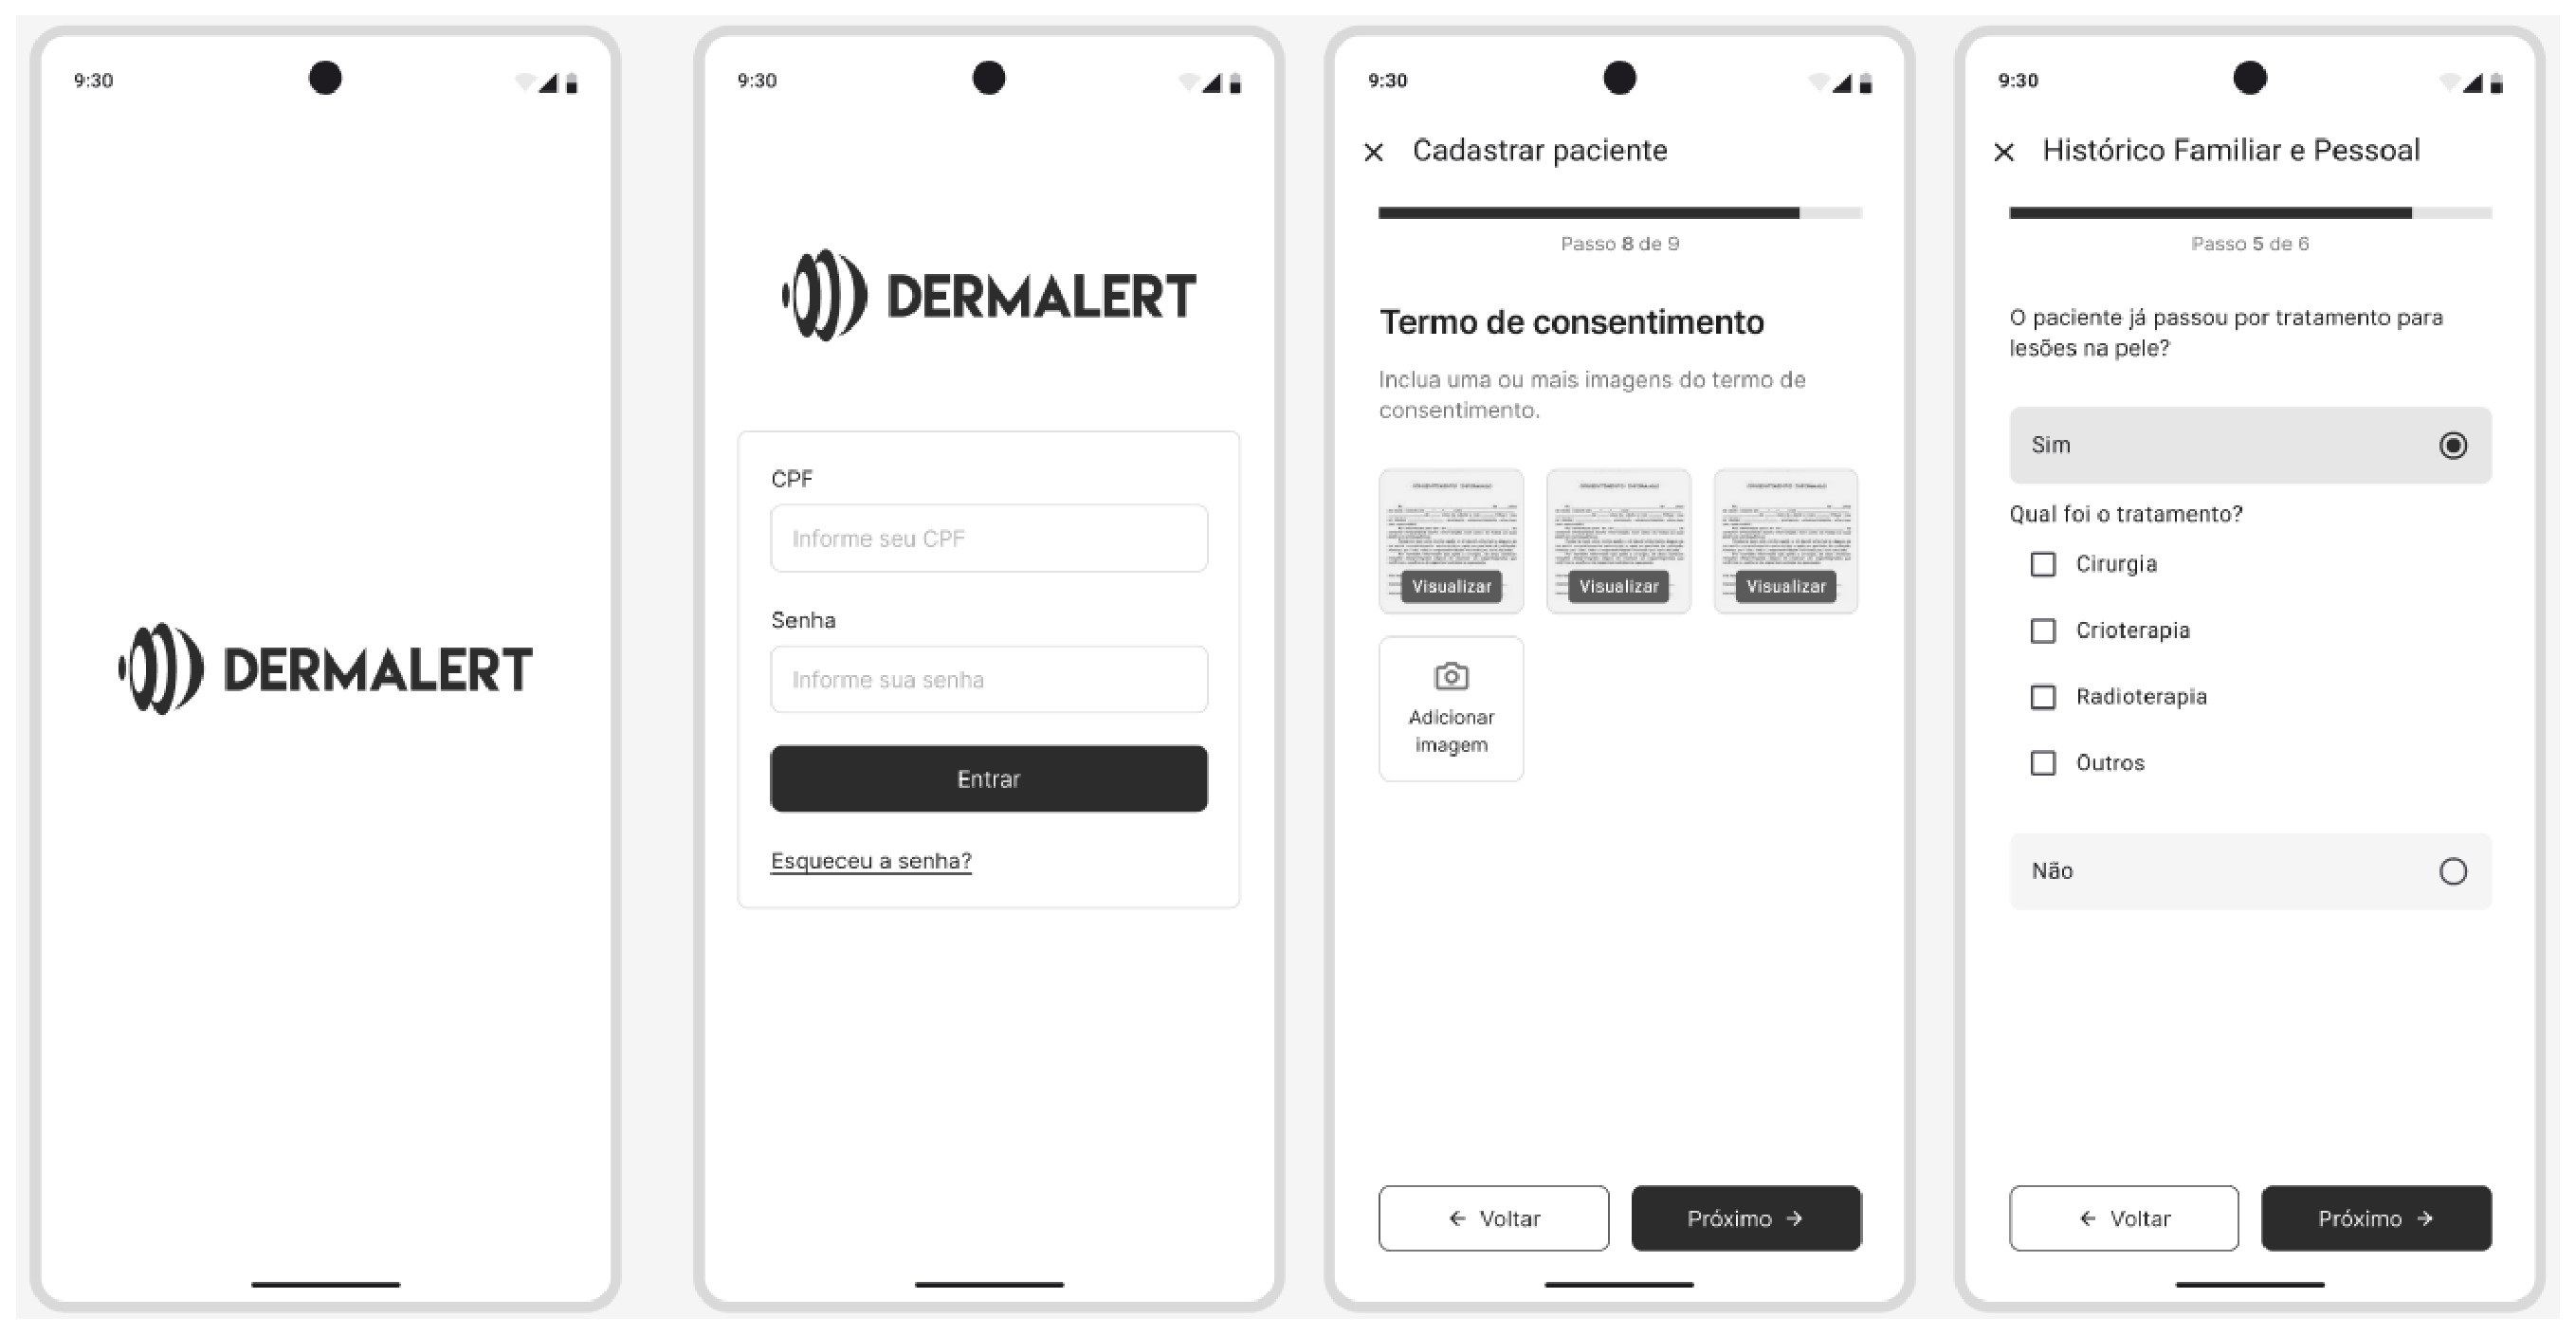
\includegraphics[width=0.8\textwidth]{figuras/app_screenshot.eps}
\caption{Tela de cadastro e coleta de dados clínicos no aplicativo DermAlert}
\label{fig:tela_cadastro_paciente}
\end{figure}

Lorem ipsum dolor sit amet, consectetur adipiscing elit. Sed do eiusmod tempor incididunt ut labore et dolore magna aliqua. Ut enim ad minim veniam, quis nostrud exercitation ullamco laboris nisi ut aliquip ex ea commodo consequat. Duis aute irure dolor in reprehenderit in voluptate velit esse cillum dolore eu fugiat nulla pariatur. Excepteur sint occaecat cupidatat non proident, sunt in culpa qui officia deserunt mollit anim id est laborum.
\begin{figure}[H]
\centering
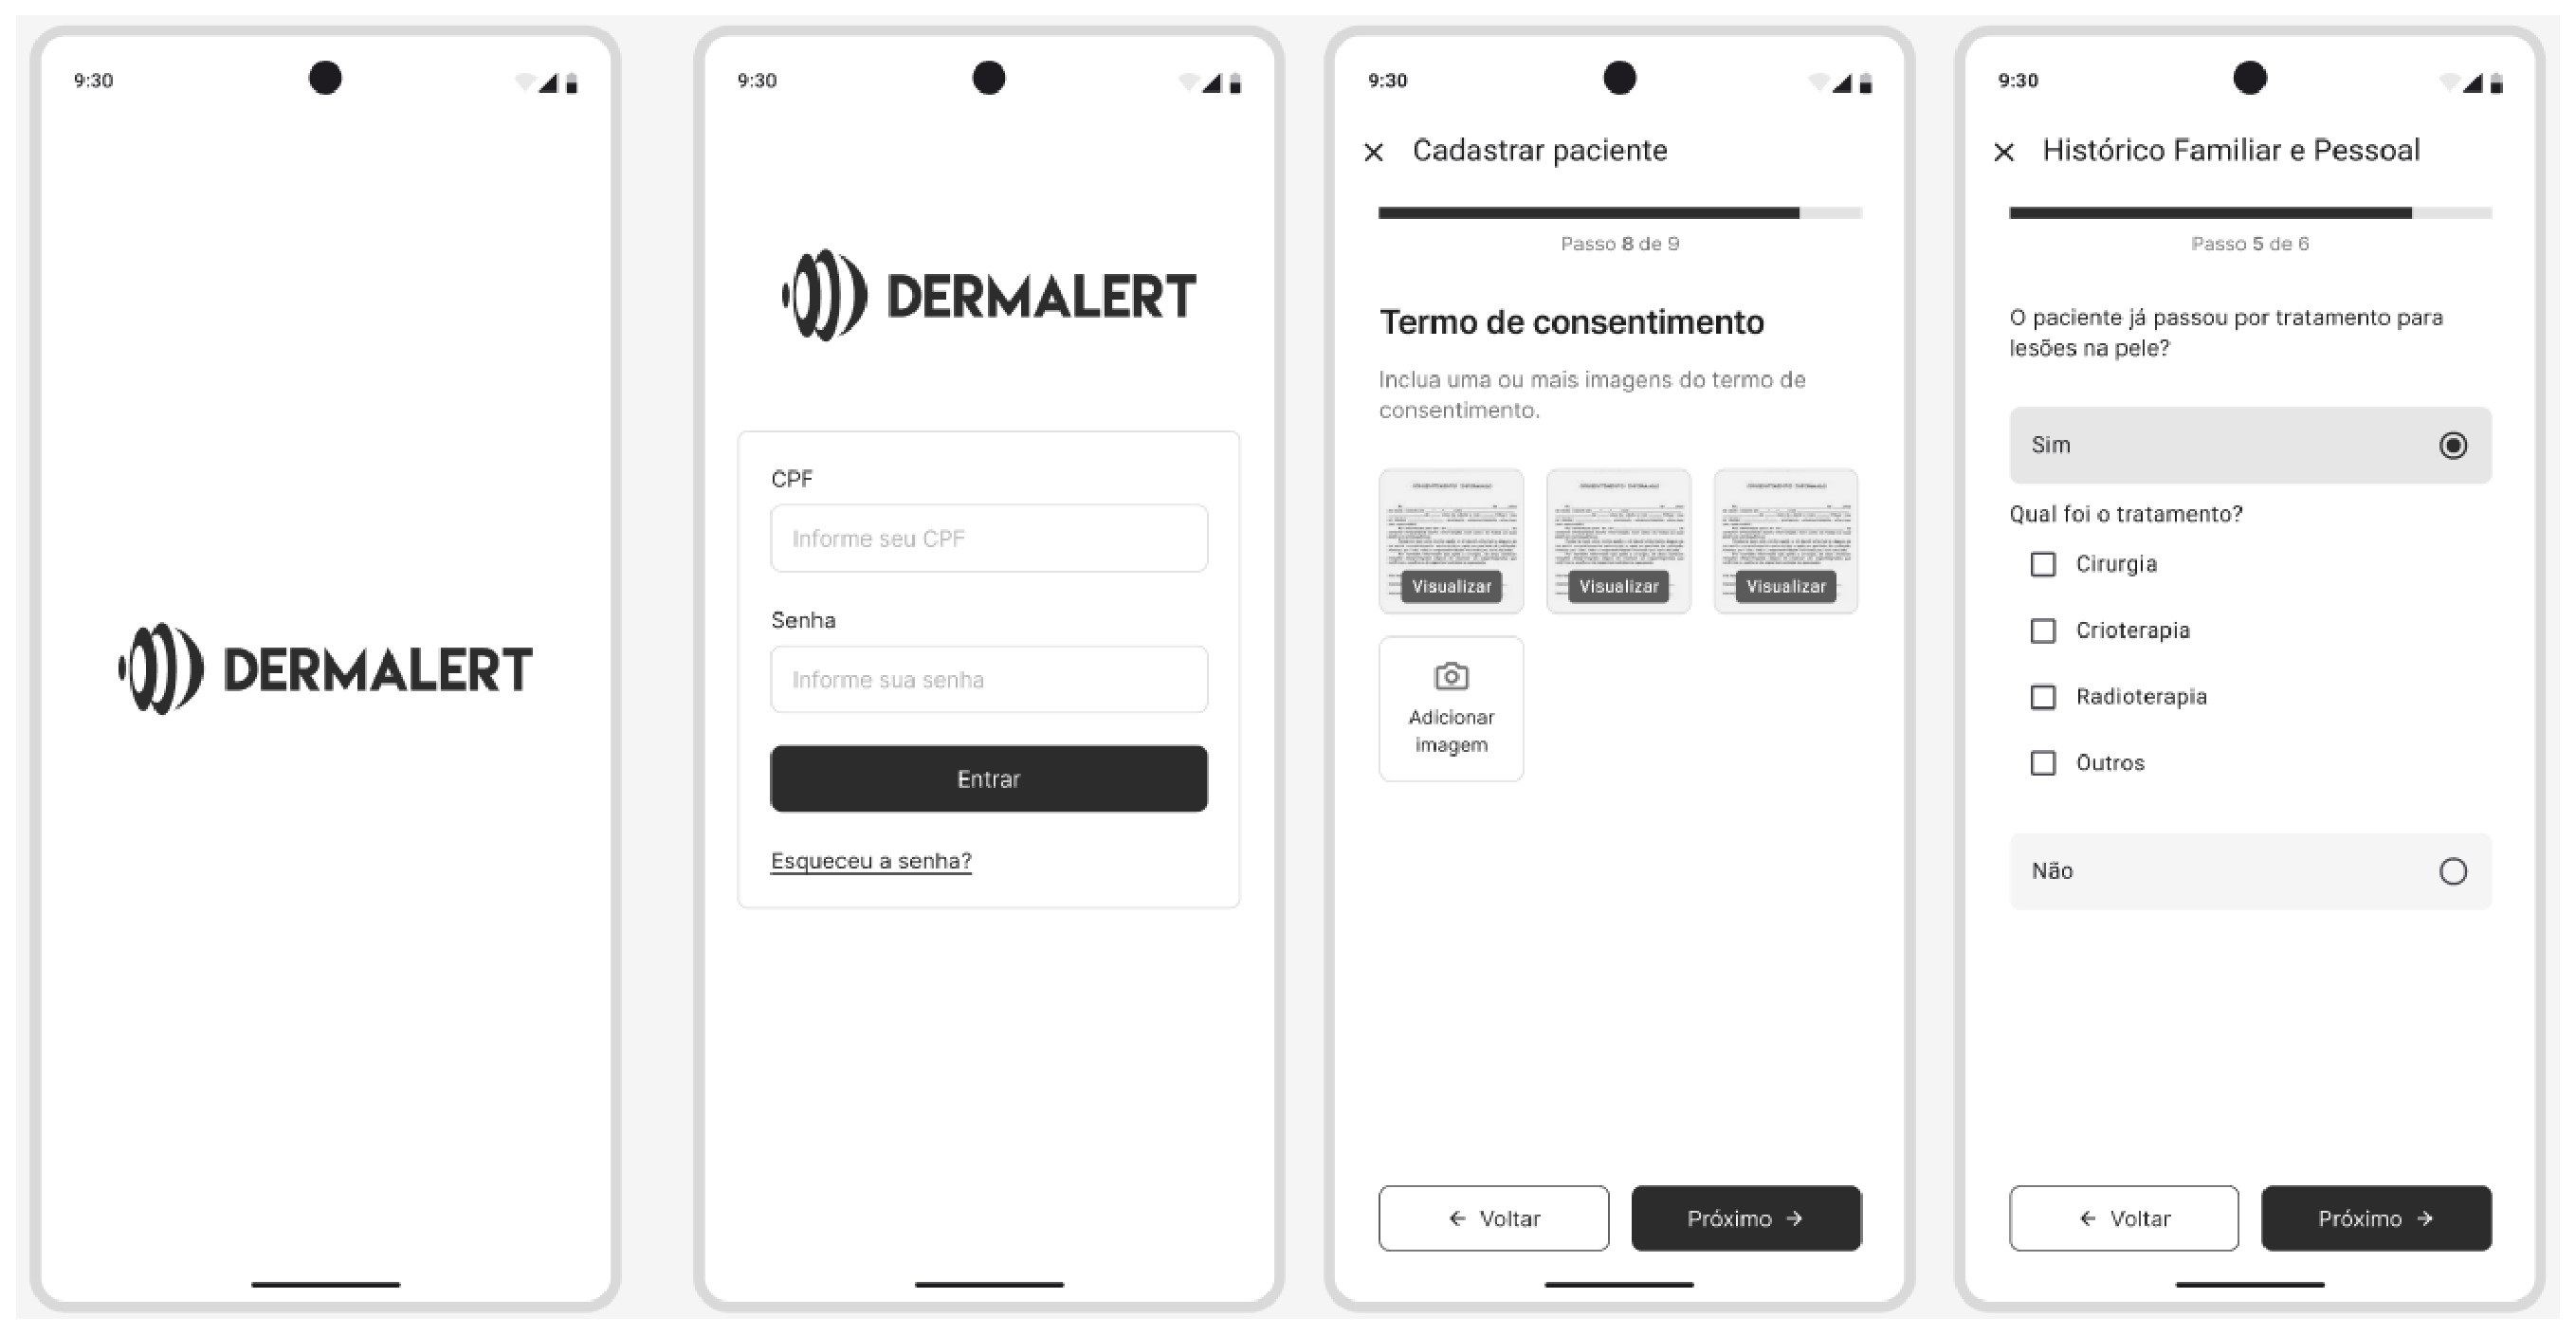
\includegraphics[width=0.8\textwidth]{figuras/app_screenshot.eps}
\caption{Listagem de imagens dermatológicas coletadas com metadados estruturados}
\label{fig:tela_listagem_imagens}
\end{figure}

Lorem ipsum dolor sit amet, consectetur adipiscing elit. Sed do eiusmod tempor incididunt ut labore et dolore magna aliqua. Ut enim ad minim veniam, quis nostrud exercitation ullamco laboris nisi ut aliquip ex ea commodo consequat. Duis aute irure dolor in reprehenderit in voluptate velit esse cillum dolore eu fugiat nulla pariatur. Excepteur sint occaecat cupidatat non proident, sunt in culpa qui officia deserunt mollit anim id est laborum.
\begin{figure}[H]
\centering
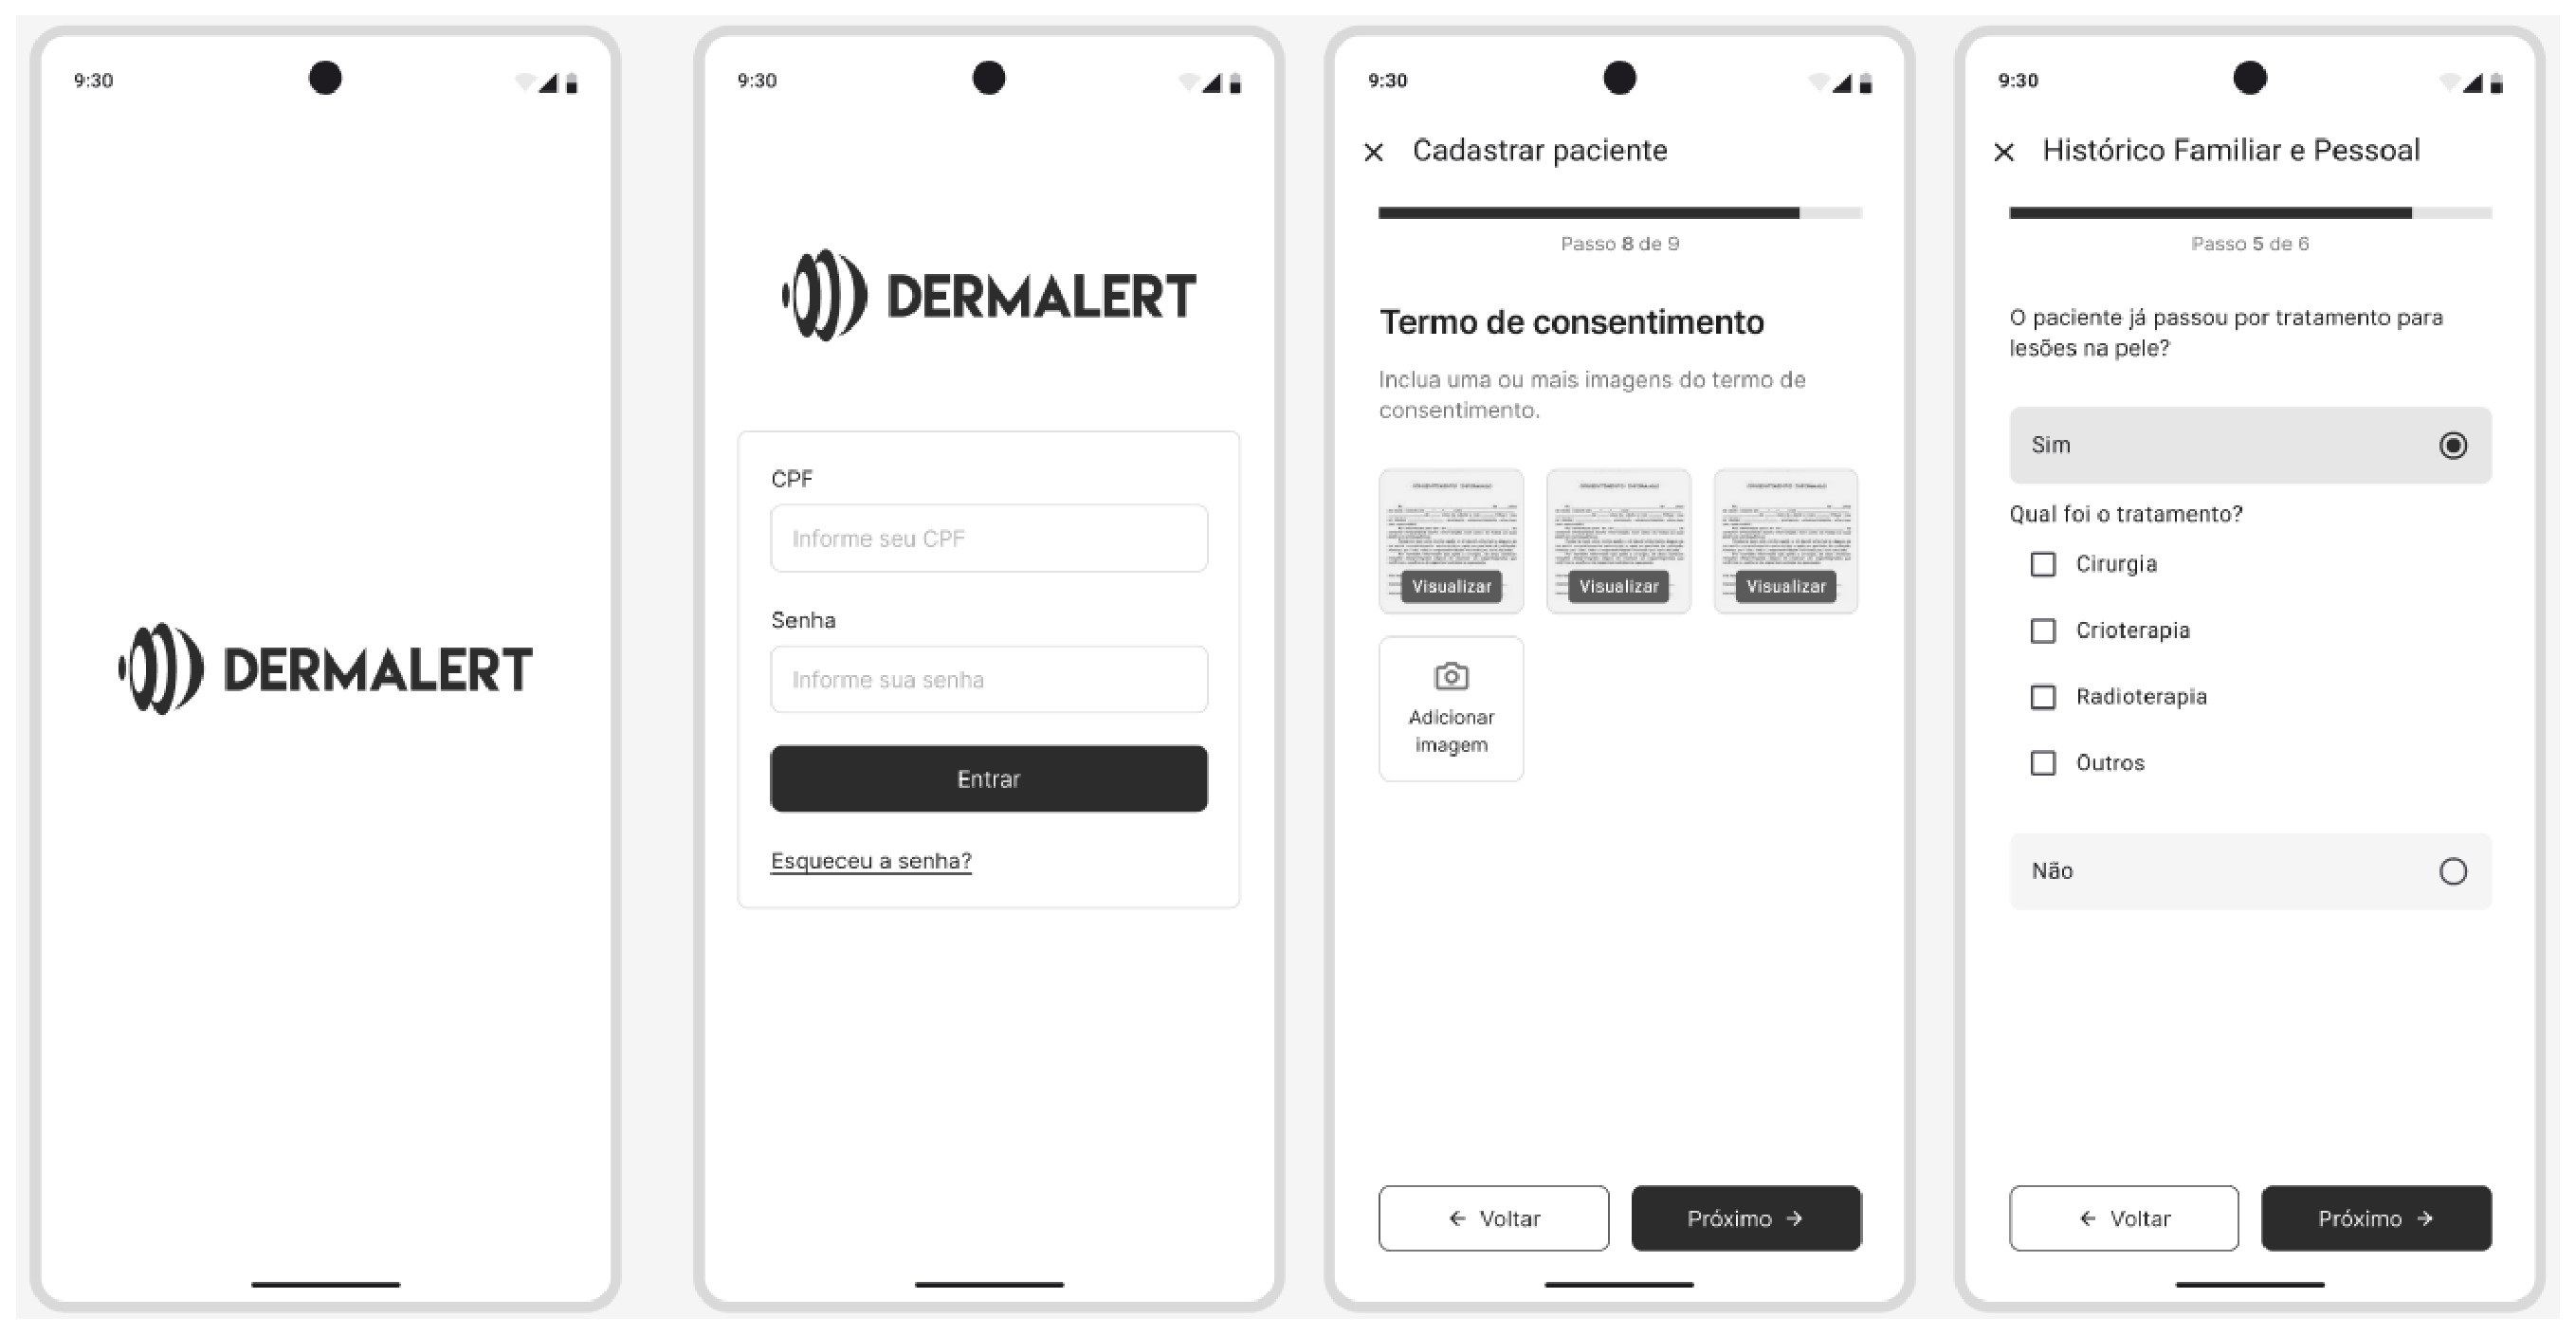
\includegraphics[width=0.8\textwidth]{figuras/app_screenshot.eps}
\caption{Dashboard inicial para visualização de dados e acompanhamento de ingestão}
\label{fig:dashboard_analises}
\end{figure}


\section{Evoluções Futuras}
Com base na arquitetura completa proposta, algumas funcionalidades planejadas para uma futura versão da plataforma incluem o desenvolvimento de filtros personalizados para facilitar a criação de novos datasets com base em critérios específicos definidos pelo usuário. Também está planejada a ampliação do suporte a diferentes tipos de conexões com novas fontes de dados, aumentando a flexibilidade e a abrangência da plataforma. Outro avanço será a implementação de um modelo de permissões baseado em RBAC (Role-Based Access Control), permitindo um controle mais refinado de acesso aos dados e datasets. Por fim, o suporte ao mapeamento e relacionamento entre tabelas de uma mesma fonte, possibilitando análises mais completas e estruturadas dentro do próprio contexto da origem dos dados.

\section{Conclusão}
O uso de dados de saúde em aplicações de machine learning apresenta desafios significativos relacionados à fragmentação das fontes, heterogeneidade semântica, viés nos dados e requisitos rigorosos de segurança e privacidade. No contexto do diagnóstico dermatológico, essas limitações afetam diretamente a eficácia dos modelos preditivos, sobretudo em populações sub-representadas. A coleta e integração sistemática de dados clínicos e imagens de lesões, respeitando princípios de governança e diversidade, torna-se essencial para o desenvolvimento de algoritmos mais justos, confiáveis e clinicamente relevantes. Assim, este trabalho parte do desafio de construir uma infraestrutura capaz de orquestrar esses dados de forma ética e interoperável, viabilizando avanços em inteligência artificial aplicada à saúde pública.

O desenvolvimento da plataforma DermAlert representa um avanço significativo na aplicação de arquitetura Data Fabric para o contexto dermatológico brasileiro, pois combina uma arquitetura resiliente e adaptável às condições de infraestrutura desafiadoras do sistema de saúde, uma camada de integração semântica que resolve a heterogeneidade terminológica entre instituições e uma demonstração prática de como tecnologias open-source podem ser ajustadas para criar soluções especializadas de baixo custo voltadas à saúde pública. Além de disponibilizar a infraestrutura, a plataforma possui um aplicativo para a aquisição de imagens de lesões de pele e metadados da lesão do paciente. Essa nova base de dados, respeitando os padrões internacionais e disponibilizada no Data Fabric, contribui com a comunidade científica com uma diversidade de tons de pele, possibilitando o treinamento de modelos de machine learning mais adaptados para a realidade da população brasileira.
Trabalhos futuros incluem expansão para outras subespecialidades dermatológicas além de lesões oncológicas, como dermatoses inflamatórias e infecciosas. Estamos desenvolvendo capacidade de análise longitudinal para acompanhamento automático de evolução de lesões ao longo do tempo e integrando modelos de risco personalizado baseados em fatores genéticos e ambientais.

Uma oportunidade particularmente promissora é a implementação de federação de aprendizado, permitindo que modelos sejam treinados em dados distribuídos sem necessidade de centralização, endereçando importantes preocupações de privacidade.
